\documentclass[tikz,border=5pt]{standalone}
\usepackage[T1]{fontenc}
\usepackage{lmodern,amsmath,amssymb}
\usetikzlibrary{arrows.meta,calc,positioning,fit,backgrounds,shapes.geometric,matrix,decorations.pathreplacing,patterns}
\definecolor{ink}{gray}{0.08}
\definecolor{wash}{gray}{0.965}
\definecolor{soft}{gray}{0.45}
\tikzset{box/.style={draw=ink,line width=.65pt,fill=white,align=center,inner sep=4pt,outer sep=0pt,font=\small},flow/.style={draw=ink,line width=.65pt,-{Latex[length=1.8mm,width=1.3mm]},rounded corners=2pt},annotation/.style={font=\scriptsize,text=soft,align=center},groupbox/.style={draw=soft,dashed,line width=.45pt,fill=wash}}
\begin{document}
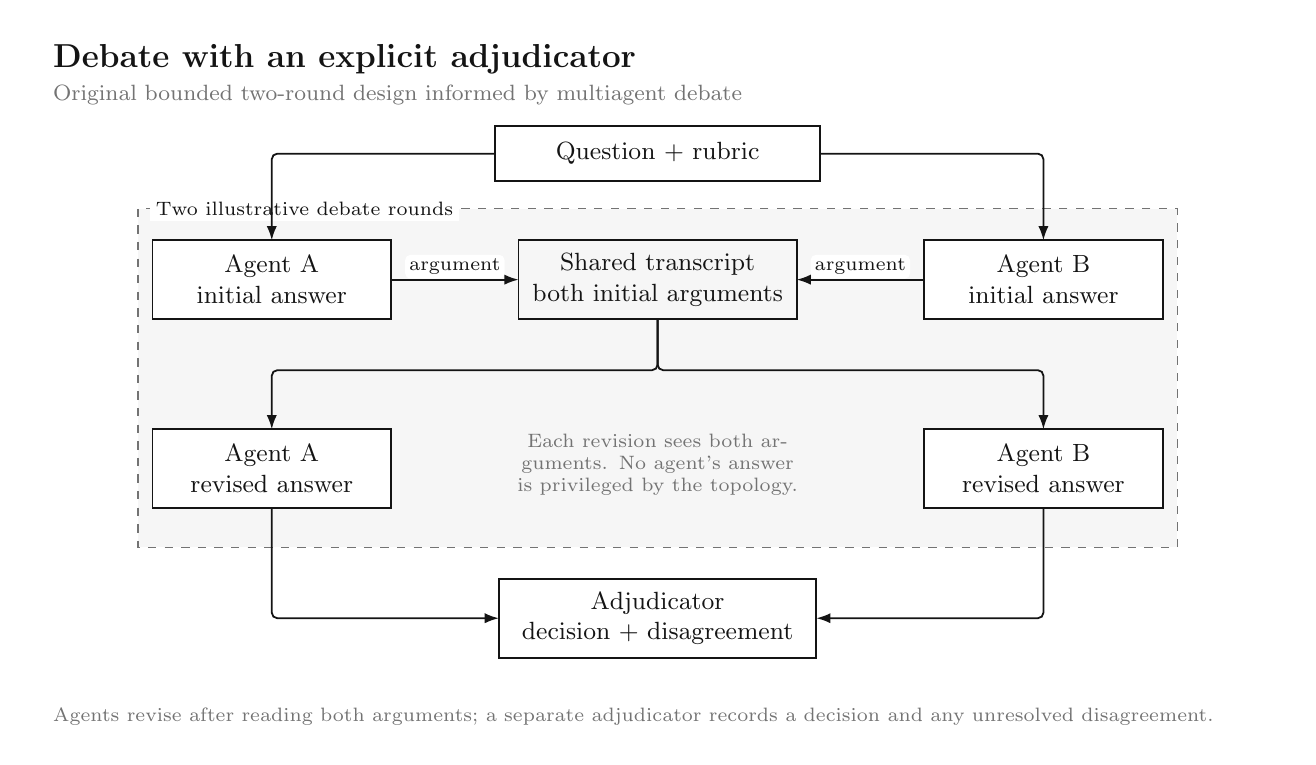
\begin{tikzpicture}[x=1cm,y=-1cm,font=\rmfamily,text=ink]

\path[use as bounding box] (0,0) rectangle (16,9);
\node[anchor=west,font=\large\bfseries] at (.2,.4) {Debate with an explicit adjudicator};
\node[anchor=west,font=\footnotesize,text=soft] at (.2,.85) {Original bounded two-round design informed by multiagent debate};
\begin{pgfonlayer}{background}
\draw[groupbox] (1.4,2.3) rectangle (14.6,6.6);
\node[anchor=west,font=\scriptsize,fill=white,inner sep=2pt] at (1.5499999999999998,2.3) {Two illustrative debate rounds};
\end{pgfonlayer}
\node[box,minimum width=4.1cm,minimum height=0.7cm,text width=3.8499999999999996cm] (question) at (8,1.6) {Question + rubric};
\node[box,minimum width=3.0cm,minimum height=1.0cm,text width=2.75cm] (a0) at (3.1,3.2) {Agent A\\initial answer};
\node[box,minimum width=3.0cm,minimum height=1.0cm,text width=2.75cm] (b0) at (12.9,3.2) {Agent B\\initial answer};
\node[box,fill=wash,minimum width=3.5cm,minimum height=1.0cm,text width=3.25cm] (transcript) at (8.0,3.2) {Shared transcript\\both initial arguments};
\node[box,minimum width=3.0cm,minimum height=1.0cm,text width=2.75cm] (a1) at (3.1,5.6) {Agent A\\revised answer};
\node[box,minimum width=3.0cm,minimum height=1.0cm,text width=2.75cm] (b1) at (12.9,5.6) {Agent B\\revised answer};
\node[box,minimum width=4.0cm,minimum height=1.0cm,text width=3.75cm] (judge) at (8.0,7.5) {Adjudicator\\decision + disagreement};
\begin{pgfonlayer}{background}
\draw[flow] (question.west) -- (3.1,1.6) -- (a0.north);
\draw[flow] (question.east) -- (12.9,1.6) -- (b0.north);
\draw[flow] (a0.east) -- (transcript.west) node[midway,above,fill=white,inner sep=1.5pt,font=\scriptsize] {argument};
\draw[flow] (b0.west) -- (transcript.east) node[midway,above,fill=white,inner sep=1.5pt,font=\scriptsize] {argument};
\draw[flow] (transcript.south) -- (8,4.35) -- (3.1,4.35) -- (a1.north);
\draw[flow] (transcript.south) -- (8,4.35) -- (12.9,4.35) -- (b1.north);
\draw[flow] (a1.south) -- (3.1,7.5) -- (judge.west);
\draw[flow] (b1.south) -- (12.9,7.5) -- (judge.east);
\end{pgfonlayer}
\node[annotation,anchor=center,text width=4.3cm] at (8,5.55) {Each revision sees both arguments.
No agent's answer is privileged by the topology.};
\node[anchor=west,align=left,font=\scriptsize,text=soft,text width=15.6cm] at (.2,8.75) {Agents revise after reading both arguments; a separate adjudicator records a decision and any unresolved disagreement.};
\end{tikzpicture}
\end{document}
